\documentclass[12pt]{article}
\usepackage{amsthm,amssymb,amsfonts,amsmath,amstext,systeme,adjustbox}
\usepackage{graphicx,float,wrapfig}
\usepackage{tabularx,enumitem}
\marginparwidth 0pt
\oddsidemargin -1.2 truecm
\evensidemargin  0pt 
\marginparsep 0pt
\topmargin -2.2truecm
\linespread{1}
\textheight 25.8 truecm
\textwidth 18.5 truecm
\newenvironment{remark}{\noindent{\bf Remark }}{\vspace{0mm}}
\newenvironment{remarks}{\noindent{\bf Remarks }}{\vspace{0mm}}
\newenvironment{question}{\noindent{\bf Question }}{\vspace{0mm}}
\newenvironment{questions}{\noindent{\bf Questions }}{\vspace{0mm}}
\newenvironment{note}{\noindent{\bf Note }}{\vspace{0mm}}
\newenvironment{summary}{\noindent{\bf Summary }}{\vspace{0mm}}
\newenvironment{back}{\noindent{\bf Background}}{\vspace{0mm}}
\newenvironment{conclude}{\noindent{\bf Conclusion}}{\vspace{0mm}}
\newenvironment{concludes}{\noindent{\bf Conclusions}}{\vspace{0mm}}
\newenvironment{dill}{\noindent{\bf Description of Dill's model}}{\vspace{0mm}}
\newenvironment{maths}{\noindent{\bf Mathematics needed}}{\vspace{0mm}}
\newenvironment{inst}{\noindent{\bf Instructions}}{\vspace{0mm}}
\newenvironment{notes}{\noindent{\bf Notes }}{\vspace{0mm}}
\newenvironment{theorem}{\noindent{\bf Theorem }}{\vspace{0mm}}
\newenvironment{example}{\noindent{\bf Example }}{\vspace{0mm}}
\newenvironment{examples}{\noindent{\bf Examples }}{\vspace{0mm}}
\newenvironment{topics}{\noindent{\bf Topics}}{\vspace{0mm}}
\newenvironment{outcomes}{\noindent{\bf Expected Learning Outcomes}}{\vspace{0mm}}
\newenvironment{lemma}{\noindent{\bf Lemma }}{\vspace{0mm}}
\newenvironment{solution}{\noindent{\it Solution}}{\vspace{2mm}}
\newcommand{\ds}{\displaystyle}
\newcommand{\un}{\underline}
\newcommand{\bs}{\boldsymbol}

\begin{document}

\baselineskip 18 pt
\begin{center}
	{\large \bf HKDSE MATH Core Sample Paper II}\\
	\vspace{2 mm}
\end{center}
\vspace{0.05cm}

\begin{enumerate}
	\item \textbf{HKDSE MATH Core Sample Paper II Q1}\\
	$(3a)^2 \cdot a^3 = $
	\begin{enumerate}
		\item[A.] $3a^5$.
		\item[B.] $6a^6$.
		\item[C.] $9a^5$.
		\item[D.] $9a^6$.
	\end{enumerate}

	\item \textbf{HKDSE MATH Core Sample Paper II Q2}\\
	If $5 - 3m = 2n$, then $m =$
	\begin{enumerate}
		\item[A.] $n$.
		\item[B.] $\dfrac{2n - 5}{3}$.
		\item[C.] $\dfrac{-2n + 5}{3}$.
		\item[D.] $\dfrac{-2n + 15}{3}$.
	\end{enumerate}

	\item \textbf{HKDSE MATH Core Sample Paper II Q3}\\
	$a^2 - b^2 + 2b - 1 =$
	\begin{enumerate}
		\item[A.] $(a - b - 1)(a + b - 1)$
		\item[B.] $(a - b - 1)(a + b + 1)$
		\item[C.] $(a - b + 1)(a + b - 1)$
		\item[D.] $(a - b + 1)(a - b - 1)$
	\end{enumerate}

	\item \textbf{HKDSE MATH Core Sample Paper II Q4}\\
	Let $p$ and $q$ be constants. If $x^2 + p(x + 5) + q \equiv (x - 2)(x + 5)$, then $q = $
	\begin{enumerate}
		\item[A.] $-25$.
		\item[B.] $-10$.
		\item[C.] $3$.
		\item[D.] $5$.
	\end{enumerate}

	\item \textbf{HKDSE MATH Core Sample Paper II Q5}\\
	Let $f(x) = x^3 + 2x^2 - 7x + 3$. When $f(x)$ is divided by $x + 2$, the remainder is 
	\begin{enumerate}
		\item[A.] 3.
		\item[B.] 5.
		\item[C.] 17.
		\item[D.] 33.
	\end{enumerate}

	\item \textbf{HKDSE MATH Core Sample Paper II Q6}\\
	Let $a$ be a constant. Solve tne equation $(x - a)(x - a - 1) = (x - a)$.
	\begin{enumerate}
		\item[A.] $x = a + 1$
		\item[B.] $x = a + 2$
		\item[C.] $x = a$ or $x = a + 1$
		\item[D.] $x = a$ or $x = a + 2$
	\end{enumerate}

	\item \textbf{HKDSE MATH Core Sample Paper II Q7}\\
	Find the range of values of $k$ such that the quadratic equation $x^2 - 6x = 2 - k$ has no real roots.
	\begin{enumerate}
		\item[A.] $k < -7$
		\item[B.] $k > -7$
		\item[C.] $k < 11$
		\item[D.] $k > 11$
	\end{enumerate}

	\item \textbf{HKDSE MATH Core Sample Paper II Q8}\\
	In the figure, the quadratic graph of $y = f(x)$ intersects the straight line $L$ at $A(1 , k)$ and $B(7 , k)$. Which of the following are true?
	\begin{enumerate}
		\item[I.] The solution of the inequality $f(x) > k$ is $x < 1$ or $x > 7$.
		\item[II.] The roots of the equation $f(x) = k$ are 1 and 7.
		\item[III.] The equation of the axis of symmetry of the quadratic graph of $y = f(x)$ is $x = 3$.
		\item[]
		\begin{enumerate}

			% \begin{wrapfigure}{}{0.25\textwidth} %this figure will be at the right
				% 	% \centering
				% 	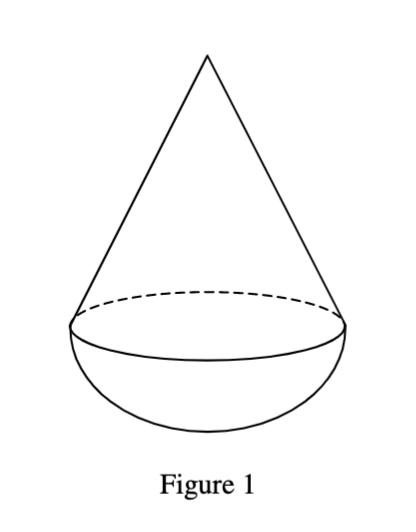
\includegraphics[width=0.25\textwidth]{SPFigure2.1}
				% \end{wrapfigure}
				\begin{minipage}{}
					\begin{enumerate}
						\item[A.] I and II only
						\item[B.] I and III only
						\item[C.] II and III only
						\item[D.] I, II and III
					\end{enumerate}
				\end{minipage}
				\begin{minipage}{.45\textwidth}
					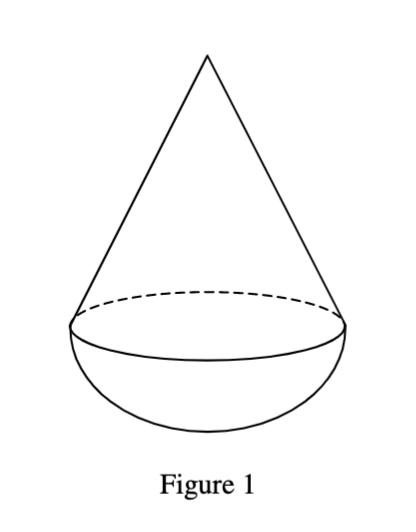
\includegraphics[scale=0.5]{SPFigure2.1}
				\end{minipage}
			\end{enumerate}
		\end{enumerate}
			
			\item \textbf{HKDSE MATH Core Sample Paper II Q9}\\
			
			
			\begin{enumerate}
				\item[A.]
				\item[B.]
		\item[C.]
		\item[D.]
	\end{enumerate}
	\item \textbf{HKDSE MATH Core Sample Paper II Q10}\\
	\begin{enumerate}
		\item[A.]
		\item[B.]
		\item[C.]
		\item[D.]
	\end{enumerate}
	\item \textbf{HKDSE MATH Core Sample Paper II Q11}\\
	\begin{enumerate}
		\item[A.]
		\item[B.]
		\item[C.]
		\item[D.]
	\end{enumerate}
	\item \textbf{HKDSE MATH Core Sample Paper II Q12}\\
	\begin{enumerate}
		\item[A.]
		\item[B.]
		\item[C.]
		\item[D.]
	\end{enumerate}
	\item \textbf{HKDSE MATH Core Sample Paper II Q13}\\
	\begin{enumerate}
		\item[A.]
		\item[B.]
		\item[C.]
		\item[D.]
	\end{enumerate}
	\item \textbf{HKDSE MATH Core Sample Paper II Q14}\\
	\begin{enumerate}
		\item[A.]
		\item[B.]
		\item[C.]
		\item[D.]
	\end{enumerate}
	\item \textbf{HKDSE MATH Core Sample Paper II Q15}\\
	\begin{enumerate}
		\item[A.]
		\item[B.]
		\item[C.]
		\item[D.]
	\end{enumerate}
	\item \textbf{HKDSE MATH Core Sample Paper II Q16}\\
	\begin{enumerate}
		\item[A.]
		\item[B.]
		\item[C.]
		\item[D.]
	\end{enumerate}
	\item \textbf{HKDSE MATH Core Sample Paper II Q17}\\
	\begin{enumerate}
		\item[A.]
		\item[B.]
		\item[C.]
		\item[D.]
	\end{enumerate}
	\item \textbf{HKDSE MATH Core Sample Paper II Q18}\\
	\begin{enumerate}
		\item[A.]
		\item[B.]
		\item[C.]
		\item[D.]
	\end{enumerate}
	\item \textbf{HKDSE MATH Core Sample Paper II Q19}\\
	\begin{enumerate}
		\item[A.]
		\item[B.]
		\item[C.]
		\item[D.]
	\end{enumerate}
	\item \textbf{HKDSE MATH Core Sample Paper II Q20}\\
	\begin{enumerate}
		\item[A.]
		\item[B.]
		\item[C.]
		\item[D.]
	\end{enumerate}
	\item \textbf{HKDSE MATH Core Sample Paper II Q21}\\
	\begin{enumerate}
		\item[A.]
		\item[B.]
		\item[C.]
		\item[D.]
	\end{enumerate}
	\item \textbf{HKDSE MATH Core Sample Paper II Q22}\\
	\begin{enumerate}
		\item[A.]
		\item[B.]
		\item[C.]
		\item[D.]
	\end{enumerate}
	\item \textbf{HKDSE MATH Core Sample Paper II Q23}\\
	\begin{enumerate}
		\item[A.]
		\item[B.]
		\item[C.]
		\item[D.]
	\end{enumerate}
	\item \textbf{HKDSE MATH Core Sample Paper II Q24}\\
	\begin{enumerate}
		\item[A.]
		\item[B.]
		\item[C.]
		\item[D.]
	\end{enumerate}
	\item \textbf{HKDSE MATH Core Sample Paper II Q25}\\
	\begin{enumerate}
		\item[A.]
		\item[B.]
		\item[C.]
		\item[D.]
	\end{enumerate}
	\item \textbf{HKDSE MATH Core Sample Paper II Q26}\\
	\begin{enumerate}
		\item[A.]
		\item[B.]
		\item[C.]
		\item[D.]
	\end{enumerate}
	\item \textbf{HKDSE MATH Core Sample Paper II Q27}\\
	\begin{enumerate}
		\item[A.]
		\item[B.]
		\item[C.]
		\item[D.]
	\end{enumerate}
	\item \textbf{HKDSE MATH Core Sample Paper II Q28}\\
	\begin{enumerate}
		\item[A.]
		\item[B.]
		\item[C.]
		\item[D.]
	\end{enumerate}
	\item \textbf{HKDSE MATH Core Sample Paper II Q29}\\
	\begin{enumerate}
		\item[A.]
		\item[B.]
		\item[C.]
		\item[D.]
	\end{enumerate}
	\item \textbf{HKDSE MATH Core Sample Paper II Q30}\\
	\begin{enumerate}
		\item[A.]
		\item[B.]
		\item[C.]
		\item[D.]
	\end{enumerate}
	\item \textbf{HKDSE MATH Core Sample Paper II Q31}\\
	\begin{enumerate}
		\item[A.]
		\item[B.]
		\item[C.]
		\item[D.]
	\end{enumerate}
	\item \textbf{HKDSE MATH Core Sample Paper II Q32}\\
	\begin{enumerate}
		\item[A.]
		\item[B.]
		\item[C.]
		\item[D.]
	\end{enumerate}
	\item \textbf{HKDSE MATH Core Sample Paper II Q33}\\
	\begin{enumerate}
		\item[A.]
		\item[B.]
		\item[C.]
		\item[D.]
	\end{enumerate}
	\item \textbf{HKDSE MATH Core Sample Paper II Q34}\\
	\begin{enumerate}
		\item[A.]
		\item[B.]
		\item[C.]
		\item[D.]
	\end{enumerate}
	\item \textbf{HKDSE MATH Core Sample Paper II Q35}\\
	\begin{enumerate}
		\item[A.]
		\item[B.]
		\item[C.]
		\item[D.]
	\end{enumerate}
	\item \textbf{HKDSE MATH Core Sample Paper II Q36}\\
	\begin{enumerate}
		\item[A.]
		\item[B.]
		\item[C.]
		\item[D.]
	\end{enumerate}
	\item \textbf{HKDSE MATH Core Sample Paper II Q37}\\
	\begin{enumerate}
		\item[A.]
		\item[B.]
		\item[C.]
		\item[D.]
	\end{enumerate}
	\item \textbf{HKDSE MATH Core Sample Paper II Q38}\\
	\begin{enumerate}
		\item[A.]
		\item[B.]
		\item[C.]
		\item[D.]
	\end{enumerate}
	\item \textbf{HKDSE MATH Core Sample Paper II Q39}\\
	\begin{enumerate}
		\item[A.]
		\item[B.]
		\item[C.]
		\item[D.]
	\end{enumerate}
	\item \textbf{HKDSE MATH Core Sample Paper II Q40}\\
	\begin{enumerate}
		\item[A.]
		\item[B.]
		\item[C.]
		\item[D.]
	\end{enumerate}
	\item \textbf{HKDSE MATH Core Sample Paper II Q41}\\
	\begin{enumerate}
		\item[A.]
		\item[B.]
		\item[C.]
		\item[D.]
	\end{enumerate}
	\item \textbf{HKDSE MATH Core Sample Paper II Q42}\\
	\begin{enumerate}
		\item[A.]
		\item[B.]
		\item[C.]
		\item[D.]
	\end{enumerate}
	\item \textbf{HKDSE MATH Core Sample Paper II Q43}\\
	\begin{enumerate}
		\item[A.]
		\item[B.]
		\item[C.]
		\item[D.]
	\end{enumerate}
	\item \textbf{HKDSE MATH Core Sample Paper II Q44}\\
	\begin{enumerate}
		\item[A.]
		\item[B.]
		\item[C.]
		\item[D.]
	\end{enumerate}
	\item \textbf{HKDSE MATH Core Sample Paper II Q45}\\
	\begin{enumerate}
		\item[A.]
		\item[B.]
		\item[C.]
		\item[D.]
	\end{enumerate}

\end{enumerate}
\end{document}

